\documentclass[11pt,a4paper]{ctexart}
\usepackage{amsmath,amssymb,bm}
\usepackage{graphicx}
\usepackage{booktabs}
\usepackage{geometry}
\usepackage{float}
\usepackage{caption}
\usepackage[hidelinks]{hyperref}
\usepackage{array}

\geometry{left=2.3cm,right=2.3cm,top=2.5cm,bottom=2.5cm}
\captionsetup{font=small,labelfont=bf}
\renewcommand{\figurename}{图}
\renewcommand{\tablename}{表}

\title{\bfseries 埃塞俄比亚新鲜英吉拉（injera）干燥过程中的传热传质建模与仿真}
\author{
  Alamrew B. Solomon\textsuperscript{a}，Solomon W. Fanta\textsuperscript{b,*}，\\
  Mulugeta A. Delele\textsuperscript{b}，Maarten Vanierschot\textsuperscript{c}\\[4pt]
  \small \textsuperscript{a} 埃塞俄比亚 Wollo 大学 Kombolcha 理工学院化学工程系\\
  \small \textsuperscript{b} 埃塞俄比亚 Bahirdar 大学 Bahirdar 理工学院化学与食品工程学院\\
  \small \textsuperscript{c} 比利时 KU Leuven 机械工程系，B-3000 Leuven\\
  \small \textsuperscript{*} 通讯作者邮箱：Solomon.Workneh@bdu.edu.et
}
\date{}

\begin{document}
\maketitle

\begin{center}
\small
\textit{原文：Heliyon 7 (2021) e06201，DOI: 10.1016/j.heliyon.2021.e06201}\\
\textit{本文为原文的中文翻译，供学习参考；引用时请以英文原文为准。}
\end{center}

\vspace{4pt}
\noindent\textbf{关键词：}扩散；干燥；英吉拉（injera）；数学建模；仿真

\begin{abstract}
\noindent
本文建立了一个数学模型，用以模拟英吉拉（injera）对流干燥过程中的传热与传质。采用有限元法（FEM），借助 COMSOL Multiphysics 5.5 对耦合的热量与水分偏微分方程组（PDEs）进行数值求解。为验证仿真结果，在两种空气温度（313.15 K 与 333.15 K）和两种风速（0.25 与 0.5 m\,s$^{-1}$）下，使用隧道式干燥机开展了干燥实验。预测结果与实验结果吻合良好：温度和水分比的决定系数均达到 $R^2>0.95$，水分比的均方根误差 RMSE $<0.05$，温度 RMSE $<3.5$ K。不同时刻与不同位置（厚度方向与直径方向）下英吉拉的预测温度分布与水分比分布，清晰地展示了干燥的均匀性。在温度 333.15 K、相对湿度 11\%、风速 0.5 m\,s$^{-1}$ 的条件下，将英吉拉的水分比从 1（--）降至 0.03（--）所需时间为 125 min。干燥过程中，温度与风速对水分降低均有显著影响（$p<0.05$）；二者的交互作用对英吉拉除水速率亦表现出显著差异（$p<0.05$）。
\end{abstract}

\section{引言}

英吉拉是埃塞俄比亚以及厄立特里亚、索马里和苏丹部分地区广泛食用的主粮之一（Tesfay 等，2014）。它是一种扁平的圆饼状产品，由超级谷物苔麸 \textit{Eragrostis tef} (Zucc.) Trotter、高粱、大麦或它们的混合物制成的面粉加工而成（Satheesh 和 Fanta，2018）。苔麸是埃塞俄比亚本地的热带谷物（Neela 和 Fanta，2020）。起初它并未受到太多重视，直到研究者发现苔麸不含麸质，这使其作为健康营养食品极具吸引力（Gebremariam 等，2014）。近年来，英吉拉的益处受到特别关注，许多研究对基于苔麸的食品进行了探讨（Gebremariam 等，2015）。尽管如此，英吉拉并不耐贮藏，在环境温度下存放三四天后即会因腐败霉菌而变质（Ashagrie 和 Abate，2012）。显然，采用露天日晒干燥来控制腐败的食品原料，由于环境条件不稳定、易受灰尘与虫害污染，或因吸湿回潮导致变质，并不适合大规模生产（Ertekin 和 Yaldiz，2004）。如今，科学推荐的对流干燥技术已成为保藏食品的重要手段（Tripathy 和 Kumar，2008）。围绕食品的对流气流有两个主要作用：一是传递热量以蒸发食品内部的水分，二是带走所形成的水蒸气。因此，水分含量的降低可通过抑制微生物生长或减少化学反应来促进食品保藏，而这两种过程都会导致食品品质劣变（Law 等，2016；Vásquez-Parra 等，2013）。食品干燥中同时发生的传热传质现象的建模十分复杂，因为蒸发过程涉及若干相互关联的物理现象（Datta，2007b）。因此，COMSOL Multiphysics、MATLAB 和 ANSYS 等数学工具对于求解热量、质量与动量传递方程（包括食品的多孔介质建模）而言是必不可少的（Datta，2007a）。一个有趣的耦合方程数值求解模型是计算流体力学（CFD），因为它可以同时求解流体流动与传热传质（Aregawi 等，2014a；Datta，2007b）。对数值数据进行后处理有助于描述所涉及的物理现象，进而对整体干燥工艺与产品质量进行优化（Bennamoun 等，2015；Bird 等，2015）。数值模型开发中最关键的一步是材料物性值的选取。生物材料往往具有各向异性，且并非总能忽略这种非均质性而采用整体平均条件。此外，密度、导热系数、水分扩散系数等多种物性在干燥过程中都依赖于温度、组成、湿度与时间（Berk，2018；Datta，2007a；Feyissa 等，2013）。在用于食品基质贮藏与干燥工艺设计的各类传热传质仿真中，必须纳入这些变化。因此，需要建立考虑这些变化的数学模型，才能获得准确的仿真结果（Datta，2007b）。鉴于上述重要性，本文研究的目的是考察若干数学模型在模拟英吉拉干燥过程中传热传质现象的适用性。模型结果通过比较平均含水率进行了实验验证。最后，评估了工艺温度对除水速率的影响，并确定了达到目标含水率所需的时间。

\section{数学模型的建立}

数学建模是求解干燥相关优化问题的良好工具，非常适合评估各种工艺参数（温度、风速与湿度）以及干燥时间的影响（Kumar 等，2014）。为食品建立包含相关物理现象的干燥模型是一项极具挑战性的任务，主要原因是食品结构复杂，且其材料物性在干燥过程中会发生变化。此外，干燥过程中传热与传质高度耦合，使其成为一个非常复杂的过程。因此，建模假设不可或缺，但必须审慎设定，以确保对所涉及物理过程有充分的表征（Datta，2007b）。

\subsection{控制方程}

埃塞俄比亚新鲜英吉拉干燥过程中的稳态动量传递与非稳态传热传质建模，基于牛顿定律、傅里叶定律和菲克定律建立。所采用的动量、连续性、质量与热量传递控制方程分别见式 (1)、(2)、(3) 和 (15)。

\subsubsection{动量方程}

基于动量守恒与连续性原理，待干燥产品周围静止气流的控制方程为
\begin{equation}
\rho(\bm{u}\cdot\nabla \bm{u}) = -\nabla p + \nabla\cdot\left[\mu\left(\nabla \bm{u} + (\nabla \bm{u})^{T}\right)\right],
\end{equation}
\begin{equation}
\nabla\cdot \bm{u} = 0,
\end{equation}
其中 $\rho$ 为密度（kg/m$^3$），$\mu$ 为动力黏度（Pa·s），$\bm{u}$ 为速度矢量（m\,s$^{-1}$），$p$ 为压力（Pa）（Bird 等，2001，2015）。

\subsubsection{传质方程}

菲克扩散定律可用物质的通量来表述，即单位面积上物质的输送速率（Bird 等，2015）。
\begin{equation}
\underbrace{\frac{\partial c}{\partial t}}_{\text{I}} + \underbrace{\nabla\cdot(-D\nabla c)}_{\text{II}} + \underbrace{\bm{u}_i\cdot\nabla c}_{\text{III}} = \underbrace{S_m}_{\text{IV}}
\end{equation}
式 (3) 左侧的第一、二、三项分别表示水分的累积、由扩散引起的水分输运以及由对流引起的水分输运；右侧项（$S_m$）为蒸发质量通量。水分浓度 $c$ 与湿基含水率的关系为（Law 等，2016）
\begin{equation}
c = \frac{M_{wb}\,\rho_p}{M_w},
\end{equation}
其中 $M_{wb}$ 为含水率（kg/kg 湿基），$\rho_p$ 为样品密度（kg/m$^3$），$M_w$ 为水的摩尔质量（kg/mol）。式 (3) 中的 $D$ 为扩散系数，定义为（Shen 等，2020）
\begin{equation}
D = D_{va}\,\epsilon^{3/4} S_g^{10/3},
\end{equation}
其中 $D_{va}$ 表示水蒸气--空气扩散率，$S_g$ 为气相饱和度。速度场 $\bm{u}_i$ 由达西定律给出（Datta，2007a）：
\begin{equation}
\bm{u}_i = \frac{k_i}{\mu}\Delta p,
\end{equation}
\begin{equation}
k_i = k_{ii}k_{ir},
\end{equation}
其中 $\Delta p$ 为压力梯度，$k_i$ 为流体的渗透率（见式 (7)），$k_{ii}$ 表示水或气体在完全饱和状态下的固有渗透率，$k_{ir}$ 表示水（$k_{wr}$）或气体（$k_{gr}$）的相对渗透率，其相态变化范围在 0（无相）与 1（饱和相）之间。测量食品材料的固有渗透率十分困难，可作如下合理近似
\begin{equation}
k_{wr} =
\begin{cases}
\left(\dfrac{S_w - S_{ir}}{1 - S_{ir}}\right)^3, & S_w > \dfrac{1}{1.1}\\[8pt]
0, & S_w < \dfrac{1}{1.1}
\end{cases}
\end{equation}
\begin{equation}
k_{gr} =
\begin{cases}
1 - 1.1 S_w, & S_w < \dfrac{1}{1.1}\\[6pt]
0, & S_w > \dfrac{1}{1.1}
\end{cases}
\end{equation}
其中 $S_w$ 为水饱和度，定义为 $\dfrac{M_w c}{\epsilon \rho_w}$；$S_{ir}$ 为束缚液体饱和度，据 Datta（2007b）表示为 $2.88\left(\dfrac{1}{T_{t=0}}\ln\left(\dfrac{1}{\epsilon}\right)^{0.48}\right)$。式 (3) 中的源项 $S_m$ 体现了液态水与水蒸气之间的相变（Kuznetsov 和 Nield，2013），由下式定义
\begin{equation}
S_m = K_{vap}(a_w c_{v,sat} - c),
\end{equation}
其中 $S_m$ 为样品表面蒸发引起的质量源通量（mol/(m$^3$·s)），$K_{vap}$ 为考虑强蒸发的蒸发常数（s$^{-1}$），$a_w$ 为水分活度，是干基含水率 $X_{db}$ 的函数，见式 (11)（Datta，2007a），$c_{v,sat}$ 为饱和浓度，与饱和蒸气压 $p_{v,sat}$（温度的函数）相关，见式 (13)。
\begin{equation}
a_w = \exp\left(-0.0267 X_{db}^{-1.656} + 0.0107 X_{db}^{1.51}\exp(-1.287 X_{db})\right),
\end{equation}
\begin{equation}
X_{db} = \frac{c_l + c_v}{(1-\epsilon)\rho_p},
\end{equation}
\begin{equation}
C_{v,sat} = \frac{p_{v,sat}}{RT},
\end{equation}
\begin{equation}
\begin{aligned}
p_{v,sat} = \exp\big(&-5800.2206\,T^{-1} + 1.3915 - 0.0486\,T \\
&+ 4.176\times10^{-5}T^{2} - 1.445\times10^{-8}T^{3} + 6.546\ln(T)\big),
\end{aligned}
\end{equation}
其中 $X_{db}$ 为干基水分浓度，即样品中流体与干固体基质之比；$R$ 为通用气体常数。

\subsubsection{传热方程}

固体基质中热传导通量的定律最初由 Jean-Baptiste Joseph Fourier 提出（Bird 等，2015）；包含对流的传热通用控制方程可写为（Bird，2004；Bird 等，2015）
\begin{equation}
\underbrace{(\rho C_p)_{eff}\frac{\partial T}{\partial t}}_{\text{I}} + \underbrace{\nabla\cdot(-k_{eff}\nabla T)}_{\text{II}} + \underbrace{(\rho_f)(C_{pf})\bm{u}_i\cdot\nabla T}_{\text{III}} = \underbrace{S_h}_{\text{IV}}.
\end{equation}
式 (15) 的第一、二、三、四项分别表示热量的累积、导热、对流与源项。其中 $(\rho C_p)_{eff}$ 为有效体积热容，$k_{eff}$ 为有效导热系数，$\rho_f$ 为流体密度，$C_{pf}$ 为流体的热容，分别定义如下：
\begin{equation}
(\rho C_p)_{eff} = \rho_p C_{pp} - (1-\epsilon)\rho_f c_{pf},
\end{equation}
\begin{equation}
k_{eff} = \epsilon k_p + (1-\epsilon)k_f,
\end{equation}
\begin{equation}
k_f = k_w - (k_w - k_a)X_v,
\end{equation}
\begin{equation}
\rho_f = \rho_w - (\rho_w - \rho_a)X_v,
\end{equation}
\begin{equation}
C_{pf} = C_{pw} - (C_{pw} - C_{pa})X_v.
\end{equation}
式 (16) 与 (17) 中英吉拉的孔隙率 $\epsilon$ 定义为
\begin{equation}
\epsilon = 1 - \frac{\rho_s}{\rho_b},
\end{equation}
其中 $\rho_s$ 为固体密度，$\rho_b$ 为包含空气与水的体积密度（Datta，2007b）。式 (16) 与 (17) 中的热物理性质——密度 $\rho$、导热系数 $k_p$、比热容 $C_p$——对于涉及加热与冷却过程的建模与仿真十分重要（Datta，2007a），分别由式 (22) 至 (24) 计算：
\begin{equation}
\rho = \frac{1}{\sum \dfrac{x_i}{\rho_i}},
\end{equation}
\begin{equation}
C_p = \sum_{i=1}^{n}\left(c_{p_i}X_i\right),
\end{equation}
\begin{equation}
k = \sum_{i=1}^{n}\left(k_i E_i\right),
\end{equation}
\begin{equation}
E_i = \frac{x_i/\rho_i}{\sum x_i/\rho_i}.
\end{equation}
式 (22) 至 (24) 中的下标 $i$ 表示英吉拉的各组分（蛋白质、脂肪、灰分、碳水化合物和水）。式 (15) 中由空气界面向样品的源项 $S_h$ 为蒸发潜热与质量源之积，定义为
\begin{equation}
S_h = H_{evap}M_v S_m,
\end{equation}
其中 $S_h$ 为热源（W/m$^3$），$H_{evap}$ 为蒸发潜热（J/kg），$M_v$ 为水蒸气的摩尔质量（kg/mol）。

\subsection{计算域及初始与边界条件}

英吉拉的计算域、边界条件与初始条件如图~\ref{fig:1} 所示。在入口 (1) 处，干热空气沿 $x$ 方向进入通道，施加均匀的速度与温度分布，并令水蒸气浓度为零（$\bm{u}=\bm{u}_{t=0}$，$T=T_{t=0}$，$c_v=0$）。在通道出口 (4) 处采用充分发展流动条件（$\dfrac{\partial c}{\partial n}=\dfrac{\partial T}{\partial n}=0$，$n$ 为边界法向）。顶部 (5) 与底部 (6) 壁面采用无滑移、绝热条件（$u=v=w=0$，$\dfrac{\partial T}{\partial n}=\dfrac{\partial c}{\partial n}=0$）。样品域内的初始温度与浓度分别为 298.15 K 和 49\,750 mol/m$^3$。

\begin{table}[H]
\centering
\caption{初始与常数输入参数}
\label{tab:1}
\begin{tabular}{lll}
\toprule
符号 & 数值（单位） & 来源 \\
\midrule
$p_{t=0}$ & 1 atm & 本研究 \\
$c_{t=0}$ & $\dfrac{S_l\rho_w\epsilon}{M_w}=49\,750$ mol/m$^3$ & 本研究 \\
$T_{t=0}$ & 323.15 与 333.15 K & 本研究 \\
$U_{t=0}$ & 0.25 与 0.5 m\,s$^{-1}$ & 本研究 \\
$D_{wa}$ & 2.6e-5 m$^2$/s & (Cengel 和 Ghajar，2011) \\
$D_{va}$ & 2.6e-5 m$^2$/s & (Cengel 和 Ghajar，2011) \\
$H_{evap}$ & 2.454e+6 J/kg & (Kumar 等，2014) \\
$\epsilon$ & 0.74 & 本研究 \\
\bottomrule
\end{tabular}
\end{table}

\begin{table}[H]
\centering
\caption{英吉拉、空气与水的热物理性质}
\label{tab:2}
\begin{tabular}{lll}
\toprule
符号 & 数值（单位） & 来源 \\
\midrule
\multicolumn{3}{l}{\textit{密度}}\\
$\rho_{in}$ & $\rho(x,T)$ (kg/m$^3$) & 式 (22)，本研究 \\
$\rho_a$ & 1.25 kg/m$^3$ & (Karim 和 Hawlader，2005) \\
$\rho_w$ & 998 kg/m$^3$ & (Kumar 等，2014) \\
\multicolumn{3}{l}{\textit{比热容}}\\
$c_{p_{in}}$ & $c_p(x,T)$ (J/kg·K) & 式 (23)，本研究 \\
$c_{p_a}$ & 1000 J/kg·K & (Kumar 等，2014) \\
$c_{p_w}$ & 1000 J/kg·K & (Kumar 等，2014) \\
\multicolumn{3}{l}{\textit{导热系数}}\\
$k_{in}$ & $k(x,T)$ (W/m·K) & 式 (24)，本研究 \\
$k_a$ & 0.0285 W/m·K & Karim 和 Hawlader (2005) \\
$k_w$ & 0.59 W/m·K & (Cengel 和 Boles，2002) \\
\multicolumn{3}{l}{\textit{黏度}}\\
$\mu_a$ & 1.81e-5 kg/m·s & (Cengel 和 Boles，2002) \\
$\mu_w$ & 1.002e-3 kg/m·s & (Kumar 等，2014) \\
\bottomrule
\end{tabular}
\end{table}

\begin{figure}[H]
\centering
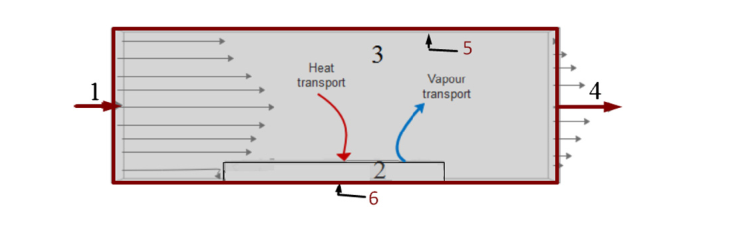
\includegraphics[width=0.95\textwidth]{figs2/fig01.png}
\caption{干燥设备二维示意图：(1) 入口，(2) 英吉拉样品，(3) 空气区，(4) 出口，(5) 顶壁，(6) 底壁。}
\label{fig:1}
\end{figure}

\subsubsection{初始条件}

英吉拉样品的初始值、常数与热物理性质见表~\ref{tab:1} 与表~\ref{tab:2}。

\subsubsection{边界条件}

基于 2.2 节与图~\ref{fig:1} 的描述，能量与质量边界条件为
\begin{equation}
\text{边界条件} =
\begin{cases}
-k\dfrac{dT}{dn} = h_T(T_s - T_a), & \text{能量边界方程}\\[8pt]
-D\dfrac{dc}{dn} = h_m(C_s - C_a), & \text{质量边界方程}
\end{cases}
\end{equation}
通道流动与英吉拉界面处的局部传热系数 $h_T$ 与传质系数 $h_m$ 由下式确定（Shen 等，2020）：
\begin{equation}
h_T =
\begin{cases}
\dfrac{2k_{eff}}{L}\dfrac{0.3387Re^{1/2}Pr^{1/3}}{\left(1+(0.0468/Pr)^{2/3}\right)^{1/3}}, & Re \ge 5\times10^{5}\\[10pt]
\dfrac{2k_{eff}}{L}Pr^{1/3}\left(0.037Re^{4/5}-871\right), & Re \le 5\times10^{5}
\end{cases}
\end{equation}
\begin{equation}
h_m = \frac{D_{air}}{L}\left(2 + 0.552R_e^{1/2}S_c^{1/3}\right),
\end{equation}
其中 $k_{eff}$ 为英吉拉的有效导热系数（W/m·K），$L$ 为特征长度（cm）。式 (28) 与 (29) 中的雷诺数 $Re$、普朗特数 $Pr$ 与施密特数 $Sc$ 可分别由式 (30) 至 (32) 表达（Yu 等，2020），其中 $\rho_a$ 为空气密度，$\mu_a$ 为空气黏度，$C_{pa}$ 为空气比热容，$D_a$ 为空气扩散率，$u_a$ 为空气速度。
\begin{equation}
Re = \frac{\rho_a u_a L}{\mu_a}
\end{equation}
\begin{equation}
Pr = \frac{C_{pa}\mu_a}{k_a}
\end{equation}
\begin{equation}
Sc = \frac{\mu_a}{\rho_a D_a}
\end{equation}

\section{材料与方法}

基于其在埃塞俄比亚苔麸种植者与使用者中的普及程度，选取 qounchote 品种，样品取自 Bahirdar 农业研究中心，并依据 Gebremariam 等（2014）的方法对英吉拉样品进行分析。

\subsection{化学成分}

英吉拉的化学成分按照公认的表列方法测定。含水率采用重量法在 378.15 K 下测定（Horwitz 等，2010；Baur 和 Ensminger，1977）；脂肪含量采用索氏抽提法测定（Kasiramar，2019）；灰分含量采用马弗炉在 823.15 K 下灼烧至无残碳测定（Baur 和 Ensminger，1977；Horwitz 等，1970）；蛋白质含量采用凯氏定氮法测定（Bradstreet，1954）；碳水化合物由差值法得到（Horwitz 等，1970）。

\subsection{干燥实验装置}

图~\ref{fig:2} 给出了实验装置示意图，腔体尺寸为 0.3$\times$0.4$\times$0.5 m，配有电加热器 (3)、鼓风机 (1)、出风腔 (8) 和电子天平 (6)。采用热电偶、热式风速仪和湿度变送器 (2,4,7) 分别测量温度、风速与相对湿度。空气由鼓风机供给，并通过风门调节风量。空气经电加热器加热，其速度由精度为 $\pm0.01$ m\,s$^{-1}$ 的热式风速仪测量，温度由精度为 $\pm1$\,$^\circ$C 的 K 型热电偶测量。空气温度设定值固定为 323.15 K 和 333.15 K，空气湿度由干湿球湿度计测定，在 323.15 K 和 333.15 K 下分别为 15.7\% 和 11\%。实验研究中，采用厚度 3 cm、直径 30 cm 的英吉拉样品进行干燥，样品初始温度为 298.15 K。样品置于由塑料网制成的托盘 (5) 上，托盘放置在强制气流系统前方，以减少托盘与样品之间的导热。每次试验约使用 100 g 物料。实验过程中持续测量样品重量，直至不再观察到明显变化为止。

\begin{figure}[H]
\centering
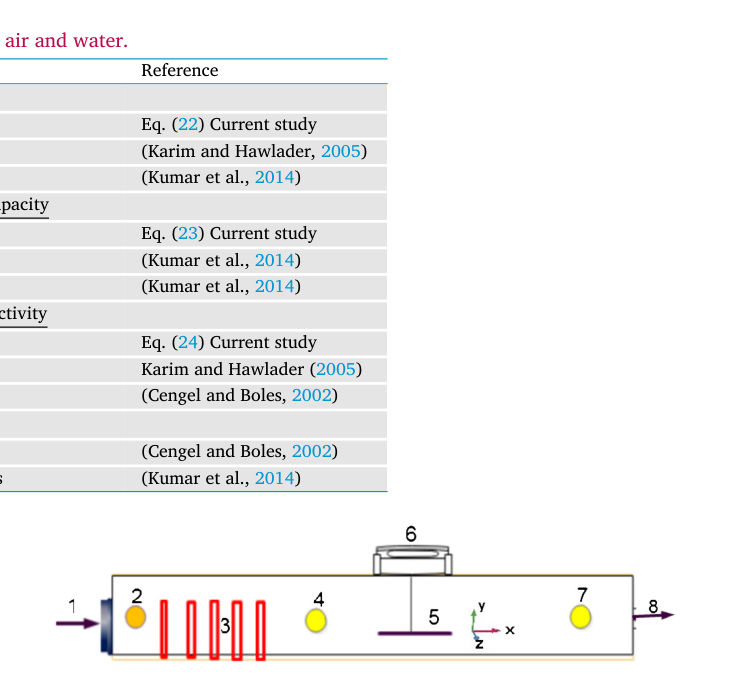
\includegraphics[width=0.5\textwidth]{figs2/fig02.png}
\caption{干燥设备二维示意图。}
\label{fig:2}
\end{figure}

\subsection{数值方法}

本研究采用商业软件 COMSOL Multiphysics（5.5 版）的有限元法求解英吉拉对流干燥中的耦合传热传质问题。选择该有限元软件是由于耦合传热传质模型的复杂性（Feyissa 等，2013）。几何定义、网格尺寸、材料性质、边界条件与物理模型均在该软件包中实现，数据求解与后处理亦使用同一软件完成。计算假定为流经英吉拉样品的层流气流，采用多波前大规模并行稀疏（Multifrontal Massively Parallel Sparse, MUMPS）直接求解器求解控制方程。仿真在本地计算机上进行，配置为 Intel(R) Core(TM) i5 处理器、2.4 GHz 主频、8.00 GB 内存，操作系统为 Windows 10（64 位）。

\subsection{网格与时间步独立性分析}

为获得可信的仿真结果，选择合适的网格与时间步尺寸十分重要。水分比（MR）的网格独立性研究从极粗网格到细网格进行，时间步长范围为 0.5 至 15 min，如图~\ref{fig:3} 所示。含水率在样品中心处测量。可以看到，水分比随网格加密而下降，直至约 400\,000 个单元后趋于稳定，继续增加单元数时解已与网格无关。图~\ref{fig:3}b 显示了时间步方面的相同机理：在较小时间步下，测得的水分比几乎保持恒定，直至某一数值（5 min），表明当时间步小于 5 min 时结果与时间步无关。

\begin{figure}[H]
\centering
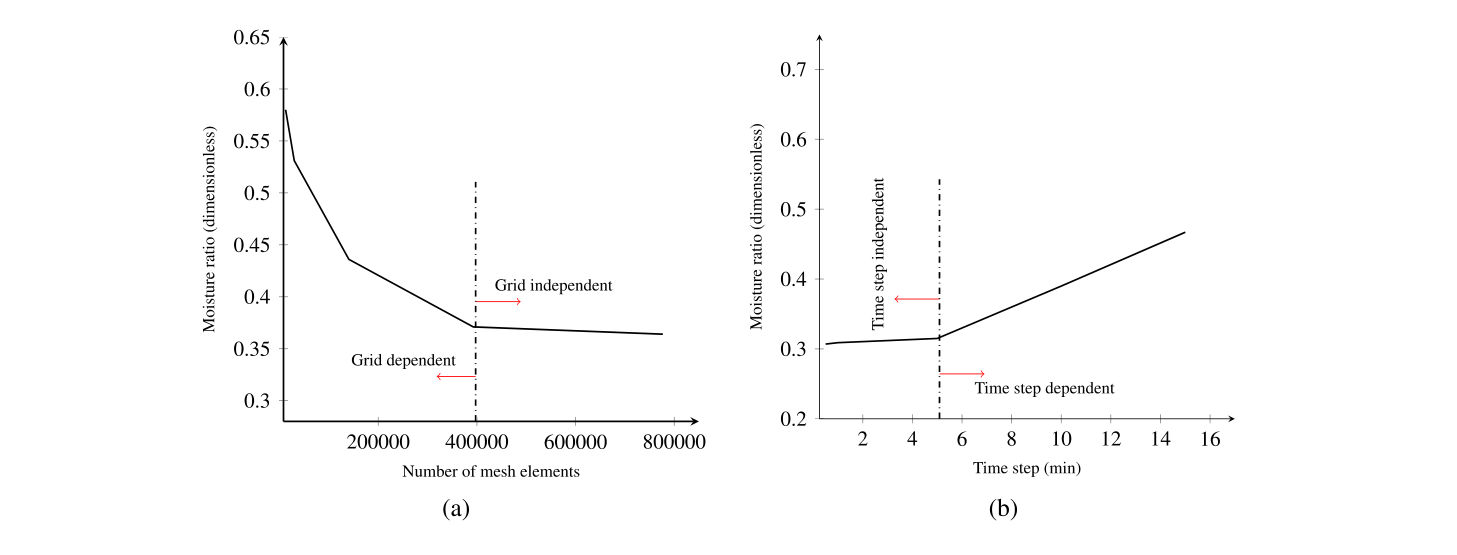
\includegraphics[width=0.95\textwidth]{figs2/fig03.png}
\caption{计算独立性分析：(a) 网格独立性；(b) 时间步独立性。}
\label{fig:3}
\end{figure}

\subsection{统计检验与验证}

干燥动力学采用大多数食品与生物材料中广泛使用的三个半经验方程进行建模，即式 (34) 的 Henderson--Pabis 模型、式 (35) 的两项（two-term）模型与式 (36) 的 Page 模型（Omolola 等，2014）。这些模型均以无量纲水分比（MR）为因变量，其定义为
\begin{equation}
MR = \frac{M_{ava} - M_e}{M_o - M_e},
\end{equation}
其中 $M_e$ 为平衡含水率，$M_{ava}$ 为 $t$ 时刻的含水率，$M_o$ 为 $t_o$ 时刻的初始含水率。

仅以风速和空气温度为变量的水分比经验关联式如下（Tunckal 和 Doymaz，2020）：
\begin{equation}
MR = \alpha_1\exp(-\alpha_2 t),
\end{equation}
\begin{equation}
MR = \beta_1\exp(-\beta_2 t) + \beta_3\exp(-\beta_4 t),
\end{equation}
\begin{equation}
MR = \exp(-\gamma_4 t^{n}).
\end{equation}
相关系数 $R^2$ 与均方根误差 RMSE 是选择描述干燥曲线最佳模型方程的主要准则。对于最佳拟合，$R^2$（Pearson 相关系数 $r$ 的平方）应较高，RMSE 应较低（Cárcel 等，2011；Demir 等，2004；Ertekin 和 Yaldiz，2004；Garau 等，2006）。为评价模型仿真的拟合优度，均方根误差与 Pearson 相关系数分别由式 (37) 与 (38) 给出。式中 $y_i$ 为第 $i$ 个预测水分比，$x_i$ 为第 $i$ 个实验水分比，$\bar{y}$ 为预测样本均值，$\bar{x}$ 为实验样本均值，$n$ 为观测次数。
\begin{equation}
RMSE = \sqrt{\frac{1}{n}\sum_{i=1}^{n}(x_i - y_i)^2}
\end{equation}
\begin{equation}
r = \frac{\sum(x_i - \bar{x})(y_i - \bar{y})}{\sqrt{\sum(x_i-\bar{x})^2(y_i-\bar{y})^2}}
\end{equation}

\section{结果与讨论}

\subsection{英吉拉的近似组成}

干燥英吉拉的碳水化合物、蛋白质、粗纤维、灰分与脂肪含量分别为 31.26$\pm$1.2 g/100 g、4.85$\pm$0.1 g/100 g、1.63$\pm$0.06 g/100 g、1.83$\pm$0.1 g/100 g 和 0.46$\pm$0.02 g/100 g。与既往报道相比，干燥英吉拉碳水化合物、蛋白质、粗纤维、灰分与脂肪含量的百分比偏差分别为 7.3、4.1、8.7、8.5、3.2 和 6.7\%，这取决于成熟度、土壤与苔麸谷物类型（Haard，1999）。英吉拉的含水率为 60.8$\pm$1.65 g/100 g，与既往工作一致，处于 60 至 65 g/100 g 的范围内（Ashagrie 和 Abate，2012）。

\subsection{热物理性质}

英吉拉的热物理性质是组成与温度的函数，而非恒定值。在 323.15 K 至 333.15 K 的温度范围内，英吉拉的密度分别为 1136.49 和 1135.41 kg/m$^3$。这表明密度随温度升高而减小，这是由于流体的分子动力学（运动）增大了空隙体积（Marcotte 等，2008）。英吉拉样品的比热容由含水量（60\%）决定，在 323.15 K 至 333.15 K 范围内为 3676 至 3675.5 J/kg·K，温度升高时并无显著变化（Shemishere 等，2018）。导热系数在 313.15 K 时取最大值 0.3657，在 333.15 K 时取最小值 0.3434 W/m·$^\circ$C。温度升高会略微降低导热系数，因为流体部分中分子间距更大、分子运动更无规，而英吉拉固体成分中的晶格振动增强。因此，导热系数随温度升高而降低（Telis-Romero 等，1998）。

\subsection{水分比与温度曲线}

图~\ref{fig:4}a 的结果清楚地显示了在入口空气温度 323.15 K 和 333.15 K、入口风速 0.5 m\,s$^{-1}$ 条件下英吉拉预测含水率与相应实验数据的对比。该图展示了典型的降速干燥阶段，且对大多数食品干燥过程而言存在一个短暂的恒速干燥阶段（Vásquez-Parra 等，2013）。在干燥初期，曲线显著下降，称为第一降速阶段，此时干燥由外部条件（暴露于干空气的面积、温度与风速）控制。在后期阶段，下降幅度较小，主要受内部传质条件（厚度与物料内部结构）控制，即所谓第二阶段。如下图所示，仿真结果与实验数据吻合良好——实验数据围绕仿真实线分布，表明该模型适合预测英吉拉的干燥行为。干燥温度升高使干燥速率显著提高，因而干燥时间缩短。在空气温度 333.15 K 下，将英吉拉含水率从初始无量纲水分比 1（--）降至最终 0.03（--）所需时间为 125 min；而在 323.15 K 下达到相同干燥效果约需 150 min。其他研究中也观察到类似结果（Hussain 和 Dincer，2003；Lemus-Mondaca 等，2013；Villa-Corrales 等，2010）。

图~\ref{fig:4}b 显示了英吉拉干燥过程中在热风温度（333.15 K 与 323.15 K）下产品温度的典型趋势。从图中可观察到三个不同阶段。在初期，产品温度低于环境空气温度，这可归因于该阶段表面水分通量迅速而产生的蒸发冷却效应：水分蒸发需要更多能量，因此初期产品接收到的热量较少。由于表面水分已被外部对流气流带走，水分因该处水势较低而由芯部向表面迁移，输运现象由内部流动条件控制。最终，体系与干燥空气温度达到平衡并保持稳态。数值仿真所得温度值与热风干燥实验测得值吻合合理（$R^2>0.95$）。存在轻微差异的原因可能在于英吉拉材料性质的信息有限或表征近似，因为这些性质在过程中会发生变化。Doymaz（2004）也报道了类似现象。

\begin{figure}[H]
\centering
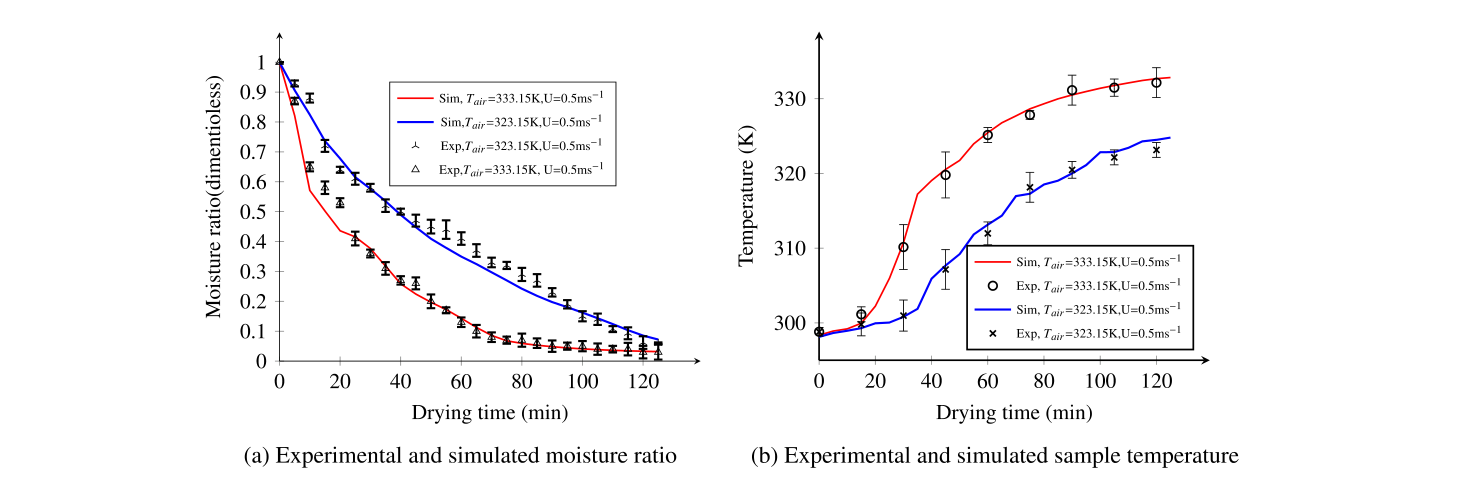
\includegraphics[width=0.95\textwidth]{figs2/fig04.png}
\caption{恒定风速（0.5 m\,s$^{-1}$）下水分比与温度的实测值与模拟值对比。}
\label{fig:4}
\end{figure}

\subsection{干燥腔内的速度分布}

图~\ref{fig:5} 展示了干燥腔内的流体流动分布。由于壁面与流体自身之间的阻力，靠近干燥腔壁面处速度值降低；在干燥腔中心观察到较高的速度值。此外，食品对流动而言相当于钝体，在其后方形成回流区。该区域内速度较低，阻碍了背面的水分排出与传热（Khan 等，2020；Pham 等，2020）。

\begin{figure}[H]
\centering
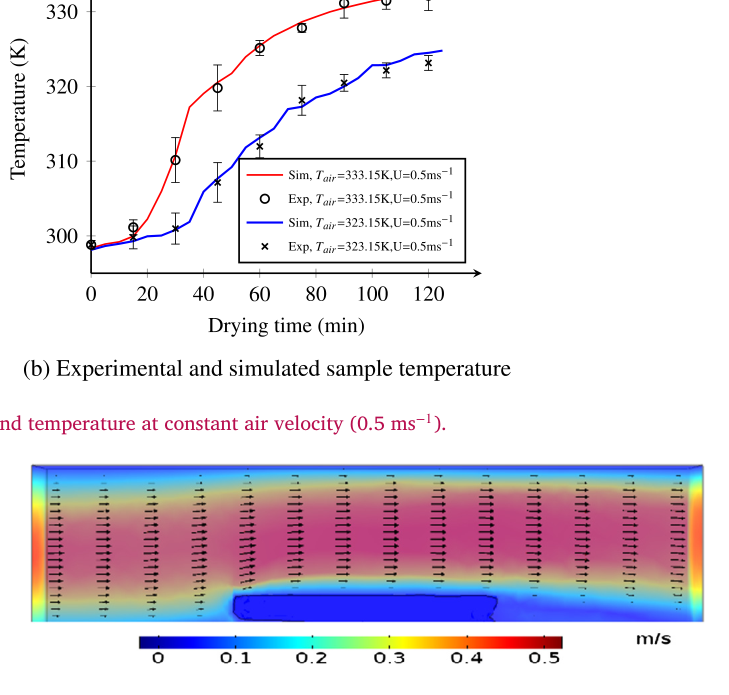
\includegraphics[width=0.5\textwidth]{figs2/fig05.png}
\caption{入口风速 0.5 m\,s$^{-1}$ 下的速度云图。}
\label{fig:5}
\end{figure}

\subsection{英吉拉表面的水分分布}

图~\ref{fig:6} 显示了不同干燥时间下英吉拉水分分布的演化。该图刻画了空气温度 333.15 K、风速 0.5 m\,s$^{-1}$ 条件下样品内部水分的演变。在初始干燥时刻（$t=0$ min），样品表面的无量纲水分分布如 图~\ref{fig:6}a 所示几乎均匀。随着干燥进行，由于英吉拉与周围空气之间的水分梯度，表面发生大量水分蒸发。此外，英吉拉样品获得了足以脱除水分的热量，在样品表面与内部芯部之间形成水分差（Datta 等，2007）。这归因于干燥过程第一阶段中大量水分由英吉拉内部蒸发至表面，并被周围空气通过对流热气流带走（图~\ref{fig:6}b 至 6e）。最终，由于高温干燥期间样品中结合水的作用使内部传质阻力显现，水分传递速率趋于停止。这导致尽管施加高温，水分向表面的迁移速率仍然下降，达到平衡含水率需要很长时间，此后不再有水分脱除（$MR=0.03$），如图~\ref{fig:6}f 所示。然而，与 333.15 K 不同，在 323.15 K 下脱除样品中剩余水分需要更多时间与能量（图~\ref{fig:7}a 至 7f）。大多数既往研究中观察到类似现象（Aregawi 等，2014a；Tzempelikos 等，2015；Villa-Corrales 等，2010）。

\begin{figure}[H]
\centering
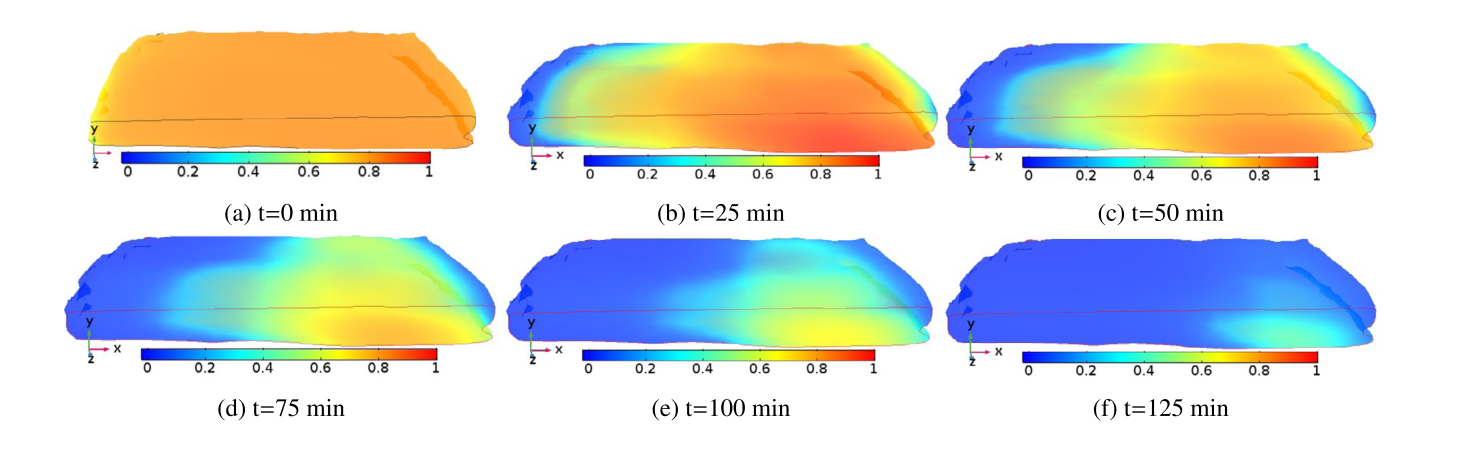
\includegraphics[width=0.95\textwidth]{figs2/fig06.png}
\caption{空气温度 333.15 K、风速 0.5 m\,s$^{-1}$ 时英吉拉样品域表面水分比分布示意图。}
\label{fig:6}
\end{figure}

\begin{figure}[H]
\centering
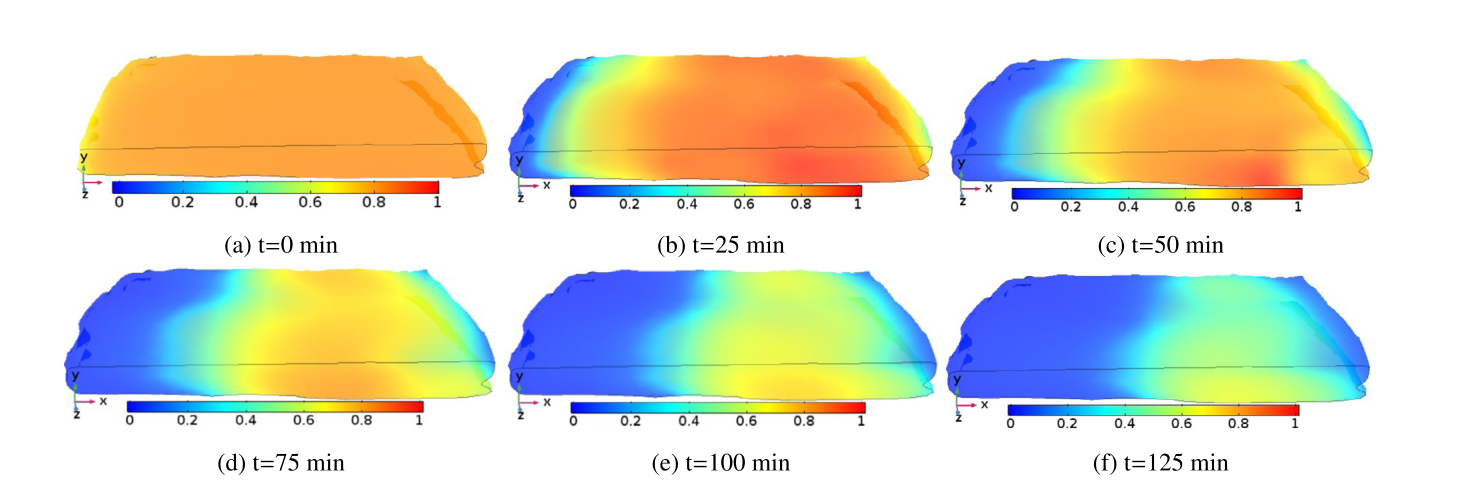
\includegraphics[width=0.95\textwidth]{figs2/fig07.png}
\caption{空气温度 323.15 K、风速 0.5 m\,s$^{-1}$ 时英吉拉样品域表面水分比分布示意图。}
\label{fig:7}
\end{figure}

\subsection{英吉拉表面的温度分布}

图~\ref{fig:8} 显示了不同干燥时间下英吉拉的温度分布，刻画了空气温度 333.15 K、风速 0.5 m\,s$^{-1}$ 条件下样品内部温度的演化。在初始干燥时刻（$t=0$ min），样品表面的温度分布几乎均匀，并与环境温度平衡（图~\ref{fig:8}a）。在干燥开始时，英吉拉表面的水分蒸发占主导，蒸发吸热阻止了样品内部升温（图~\ref{fig:8}a 至 8c）。随着干燥进行，蒸发速率下降，样品芯部逐渐升温趋向干燥空气温度（图~\ref{fig:8}e 与 8f）。研究发现，干燥温度 323.15 K 下的温度梯度（图~\ref{fig:9}a 至 9f）与图~\ref{fig:8}a 至 8f 趋势相同，只是达到平衡温度所耗时间更长。其他工作也观察到相同趋势（Aregawi 等，2014a；Villa-Corrales 等，2010）。

\begin{figure}[H]
\centering
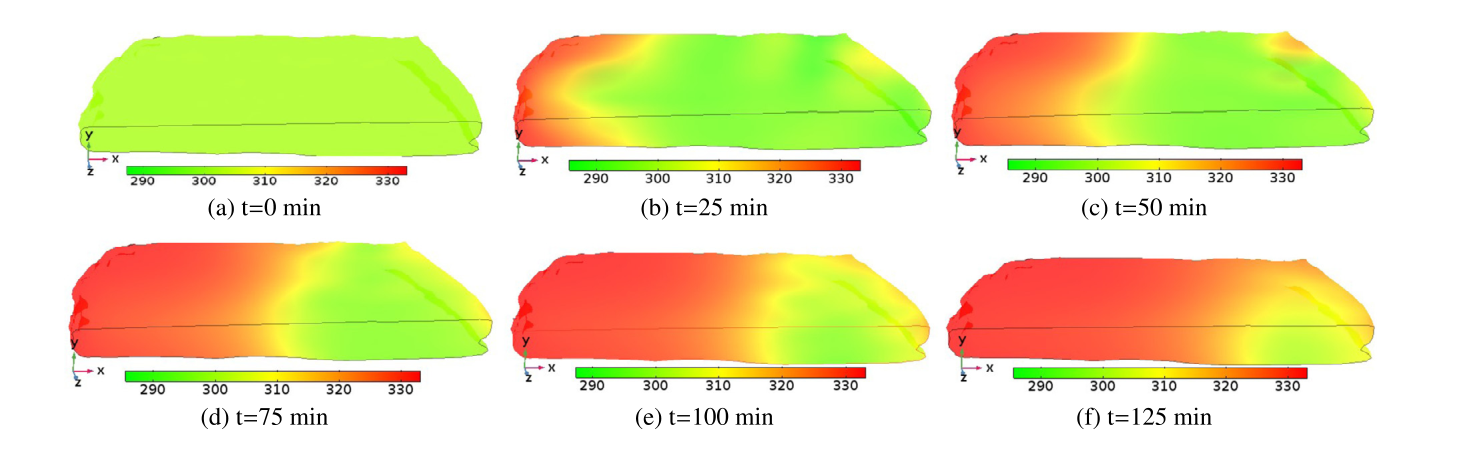
\includegraphics[width=0.95\textwidth]{figs2/fig08.png}
\caption{空气温度 333.15 K、风速 0.5 m\,s$^{-1}$ 时英吉拉样品域表面温度分布剖面示意图。}
\label{fig:8}
\end{figure}

\begin{figure}[H]
\centering
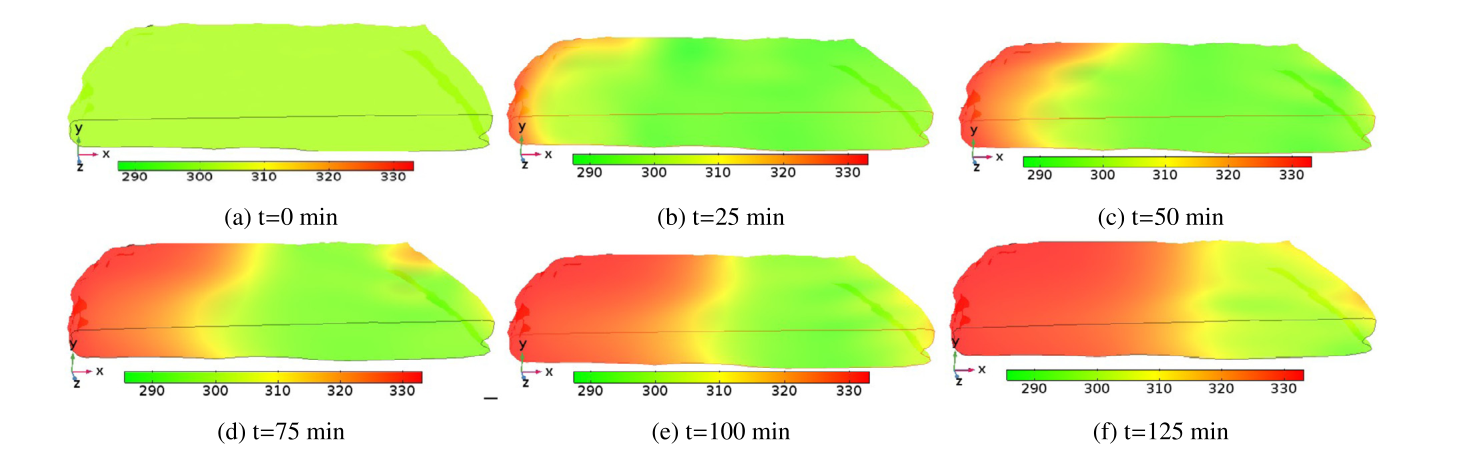
\includegraphics[width=0.95\textwidth]{figs2/fig09.png}
\caption{空气温度 323.15 K、风速 0.5 m\,s$^{-1}$ 时英吉拉样品域表面温度分布剖面示意图。}
\label{fig:9}
\end{figure}

\subsection{风速与温度对干燥速率的影响}

方差分析（ANOVA）结果表明，干燥过程中温度与风速对水分降低均有非常显著的影响（$p<1.4\times10^{-8}$）。由 ANOVA 结果可见，温度与风速之间的交互作用也表现出显著差异（$p<2.17\times10^{-5}$）。图~\ref{fig:10} 描绘了不同风速（$u=0.25$ 与 0.5 m\,s$^{-1}$）和干燥空气温度（323.15 与 333.15 K）下含水率的变化。在最初 20 min 内，由于外部干燥条件占主导，水分下降十分迅速。较高的风速与温度导致更快的水分输运速率。随着样品表面水分的对流流动增强，液态水由英吉拉内部芯部向表面的扩散及随后向空气域的蒸发均增加。Ateeque 等（2014）、Gulati 和 Datta（2013）、Zhang 和 Datta（2004）也得出类似表述。如下图所示，温度升高对干燥过程的影响强于风速增大。从图中可见，干燥初期干燥速率很高，但表面很快变干。因此，在后期阶段风速大小对蒸发的影响较小，因为表面水分含量已很低。其他研究也观察到类似行为（Pasban 等，2017；Villa-Corrales 等，2010）。

\begin{figure}[H]
\centering
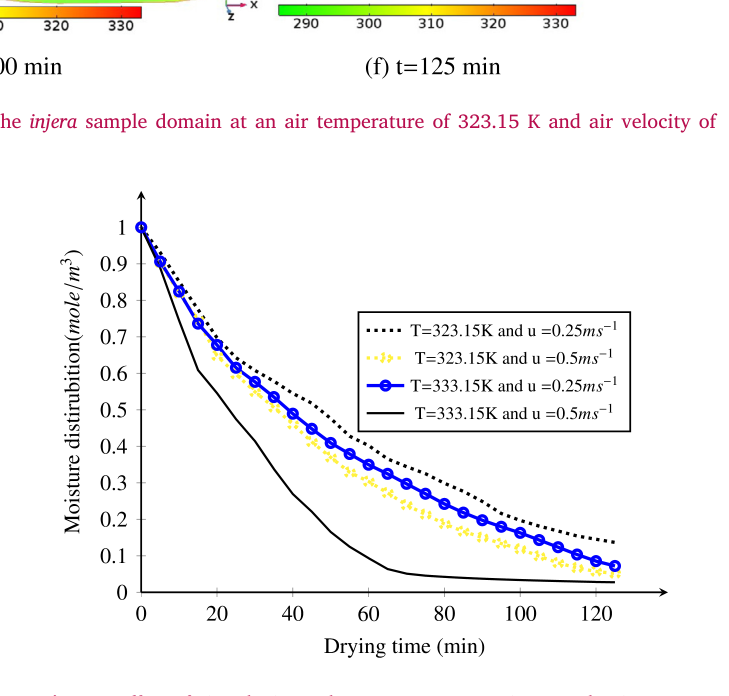
\includegraphics[width=0.5\textwidth]{figs2/fig10.png}
\caption{风速与温度对水分降低速率的影响。}
\label{fig:10}
\end{figure}

\subsection{英吉拉的有效水分扩散系数}

实验获得的英吉拉有效水分扩散系数（表~\ref{tab:3}）随风量与空气温度的升高而增大。水分扩散系数的最小值为 6.29e-9（空气温度 323.15 K、风速 0.25 m\,s$^{-1}$），最大值为 1.29e-8（空气温度 333.15 K、风速 0.5 m\,s$^{-1}$）。较高的干燥空气温度与风速由于增加了样品表面的水分损失，导致有效水分扩散系数增大。既往研究中报道了类似现象（Arslan 和 Özcan，2010；Pasban 等，2017）。

\begin{table}[H]
\centering
\caption{平均有效水分扩散系数}
\label{tab:3}
\begin{tabular}{ccc}
\toprule
$T$ (K) & $u$ (m\,s$^{-1}$) & $D_{eff}$ (m$^2$s$^{-1}$) \\
\midrule
323.15 & 0.25 & 6.29e-9 \\
323.15 & 0.5  & 7.66e-9 \\
333.15 & 0.25 & 9.21e-9 \\
333.15 & 0.5  & 1.29e-8 \\
\bottomrule
\end{tabular}
\end{table}

\subsection{水分比分布}

图~\ref{fig:11}a 展示了英吉拉干燥过程中不同位置（$y$ 坐标）与不同时刻（$t=0,20,40,\ldots,120$ min）的水分分布。该图显示了随时间增加英吉拉样品内部的水分剖面。水分随温度随时间升高而降低。由于空气与表面的温度梯度较小，这种下降在空气入口区域最大，且随样品厚度增加而梯度变大。初始时，水分在样品内均匀分布，值为 1（--），随着时间由 0 min 增至 125 min（时间间隔 20 min），逐渐降至 0.03（--）。如图所示，在 0 至 80 min 的时间范围内除水能力显著，因为样品与空气之间的水分梯度较大，导致英吉拉表面的对流蒸发占主导；80 min 之后，水分的降低由扩散主导。

图~\ref{fig:11}b 展示了不同 $x$ 坐标与时刻的水分分布。初始时，英吉拉的水分比仍然较高。随时间推移温度升高，由于该位置结合水能力下降，表面水分比降低。由于温度梯度较大，英吉拉样品内部的水分输送量很大，向中心形成显著的水分梯度。由于向中心（$x>5$ mm）尚未升温的英吉拉渗透性较低，该梯度迅速减小。在较晚时刻，温度梯度大幅减小，最终在 $t=125$ min 时温度分布几乎均匀，称为稳态温度。文献中也观察到相同行为（Pasban 等，2017；Tzempelikos 等，2015；Villa-Corrales 等，2010）。

\begin{figure}[H]
\centering
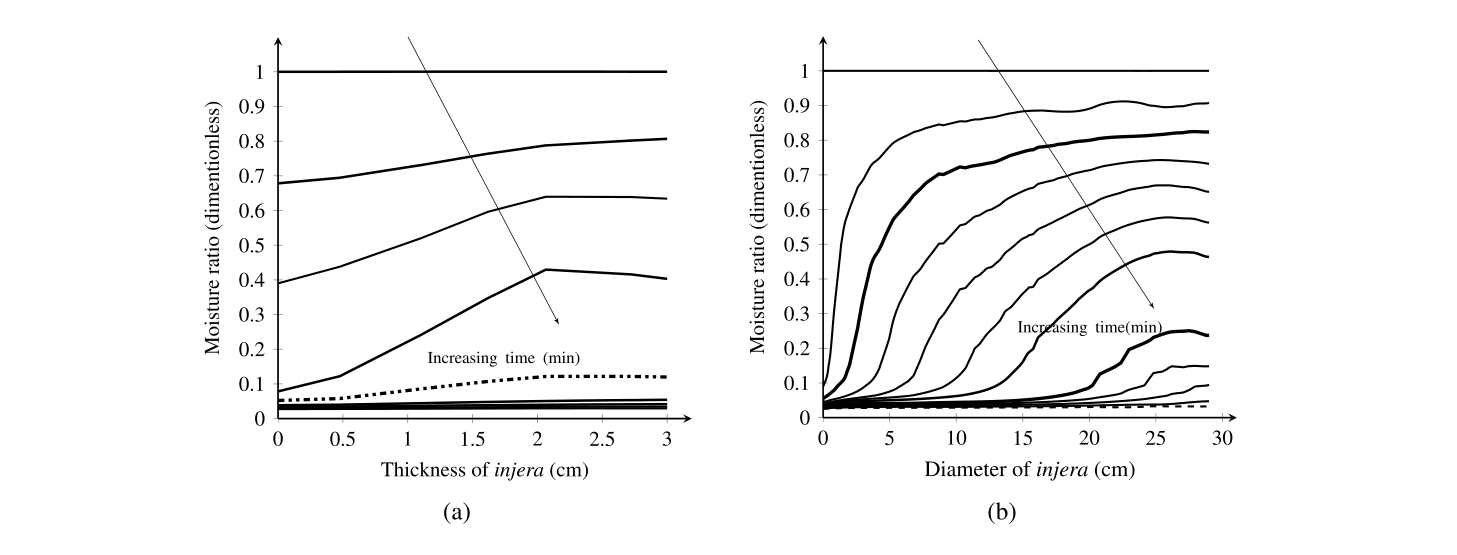
\includegraphics[width=0.95\textwidth]{figs2/fig11.png}
\caption{空气温度 333.15 K、相对湿度 11\%、风速 0.5 m\,s$^{-1}$ 时英吉拉沿厚度与直径方向（cm）的水分比分布。}
\label{fig:11}
\end{figure}

\subsection{温度分布}

图~\ref{fig:12}a 显示了英吉拉干燥过程中不同位置（$y$ 坐标）与时刻的温度分布。在干燥初期，仿真显示产品温度略有下降，但英吉拉--空气界面的顶部边界除外，其保持恒定。该现象的原因是加热吸收的能量更大，起到了入射能量汇的作用。随着干燥时间推进，由于样品表面水分被脱除，产品温度也随之升高并迅速增加。在干燥后期，其剖面保持恒定并趋于均匀，这是由于达到了稳态条件。既往研究也报道了类似效应（Aregawi 等，2014a；Datta，2007b；Tzempelikos 等，2015）。

图~\ref{fig:12}b 显示了沿直径方向的模拟温度演化。可以看出，尽管空气温度及样品与空气的接触在表面处更高，英吉拉表面的温度始终高于内部。初始时样品温度相对较低，这是由于对流与蒸发冷却降低了表面温度。Kumar 等（2012）与 Shahari（2012）的研究中也观察到类似模式。当 $x<12$ cm 时温度梯度更大，原因是热空气大部分时间滞留在样品背面，一方面增强了传热，另一方面促进了水蒸气的形成。随着干燥时间增加，产品温度也显著升高，并在样品各坐标处很快保持恒定。

\begin{figure}[H]
\centering
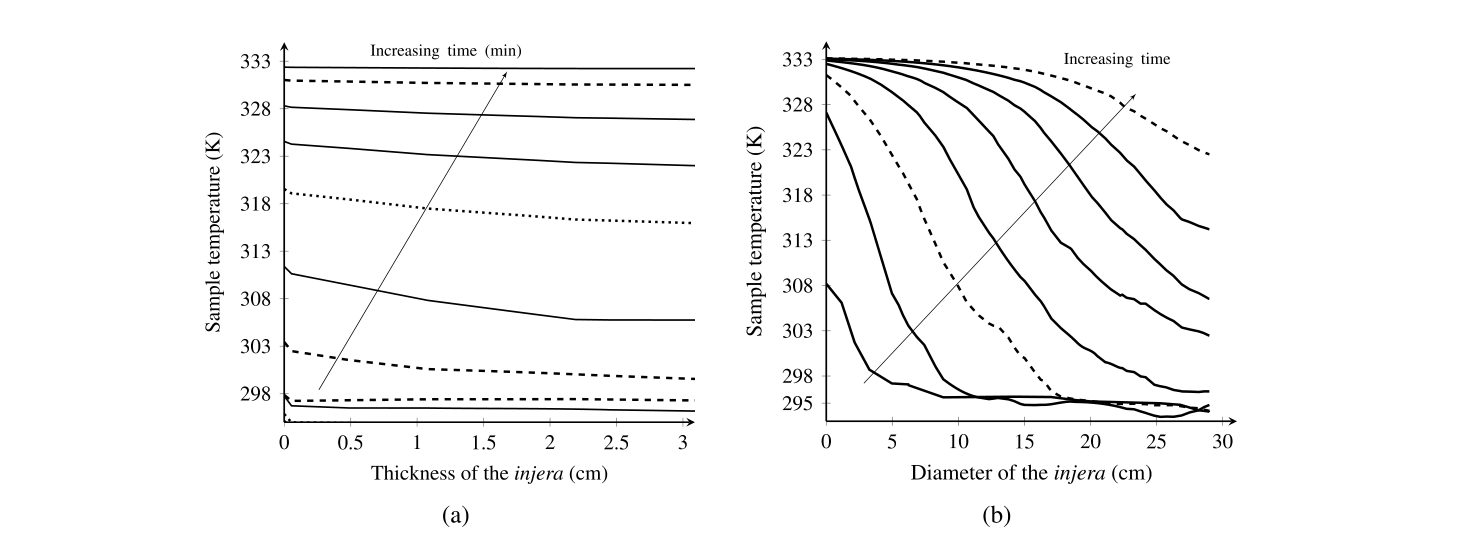
\includegraphics[width=0.95\textwidth]{figs2/fig12.png}
\caption{空气温度 333.15 K、相对湿度 11\%、风速 0.5 m\,s$^{-1}$ 时英吉拉沿厚度与直径方向（cm）的温度分布。}
\label{fig:12}
\end{figure}

\subsection{水分比与温度曲线的验证}

图~\ref{fig:13}a 展示了干燥条件为温度 333.15 K、$RH=11\%$、风速 0.5 m\,s$^{-1}$ 时的实验与数值水分值。水分比的均方根误差（RMSE）与决定系数（$R^2$）分别为 0.045 与 0.9874，这些指标反映了模型逼近实验值的程度，模型是合理可接受的。ElGamal 等（2017）与 Zielinska 和 Markowski（2010）报道了类似结果。

图~\ref{fig:13}b 比较了在总干燥时间 125 min 内每 15 min 记录的食品样品中心温度实测值与相应的模拟结果。决定系数 $R^2$ 为 0.9874，均方根误差 RMSE$=3.5$ K。这些数值表明实测温度与模拟温度吻合合理，进而说明该模型能够预测样品中心的温度分布。这些发现与 Doymaz（2004）、Zielinska 和 Markowski（2010）报道的结果一致。

\begin{figure}[H]
\centering
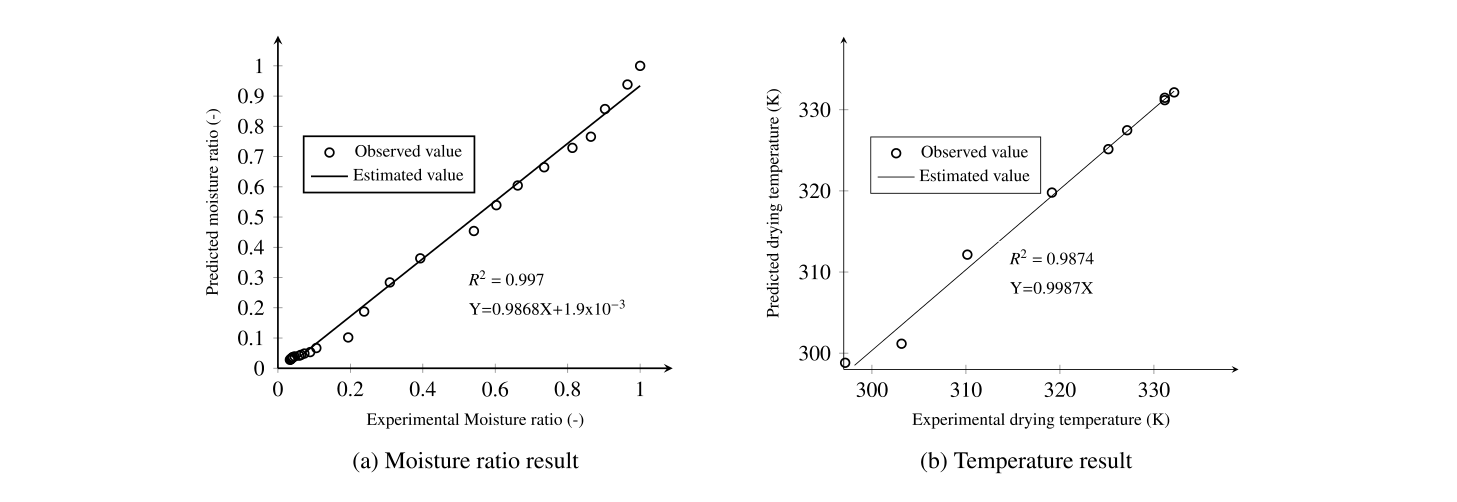
\includegraphics[width=0.95\textwidth]{figs2/fig13.png}
\caption{空气温度 333.15 K、相对湿度 11\%、风速 0.5 m\,s$^{-1}$ 时英吉拉水分比与温度的模拟值与实测值对比。}
\label{fig:13}
\end{figure}

\subsection{英吉拉与其他干燥动力学模型的比较}

图~\ref{fig:14} 比较了干燥动力学模型（Henderson--Pabis、two-term、Page）与本文英吉拉干燥过程模型。各干燥模型对干燥数据进行了拟合，并按 $R^2$ 降序、RMSE 升序排列。各干燥模型的 $R^2$ 与 RMSE 值见表~\ref{tab:4}。由这些结果可知，最佳统计结果由 Henderson--Pabis 方程获得（$R^2=0.9952$，RMSE$=0.04$），因此在图中可以看到该模型的良好逼近。在初始阶段吻合良好，然而在 80 min 之后出现显著偏差，这是由湿物料的性质影响了向表面的液体扩散输运所致。总体而言，two-term 与 Page 模型在数学模型与实验水分结果之间也表现出良好吻合，Aregawi 等（2014b）、Lemus-Mondaca 等（2013）、Tzempelikos 等（2015）也证实了这一点。该比较清楚地表明，本研究的耦合传热传质数值模型能够更好地预测英吉拉的干燥特性。

\begin{table}[H]
\centering
\caption{干燥速率（MR）随时间（min）变化的动力学建模}
\label{tab:4}
\begin{tabular}{llcc}
\toprule
模型 & 常数 & $R^2$ & RMSE \\
\midrule
Henderson \& Pabis & $\alpha=1$，$\gamma_1=-0.0189$ & 0.9952 & 0.04 \\
Two term & $\beta_1=0.875$，$\beta_2=0.135$，$\gamma_2=-0.021$，$\gamma_3=-0.0236$ & 0.9916 & 0.047 \\
Page & $\gamma_4=-0.06$，$n=0.745$ & 0.9617 & 0.087 \\
\bottomrule
\end{tabular}
\end{table}

\begin{figure}[H]
\centering
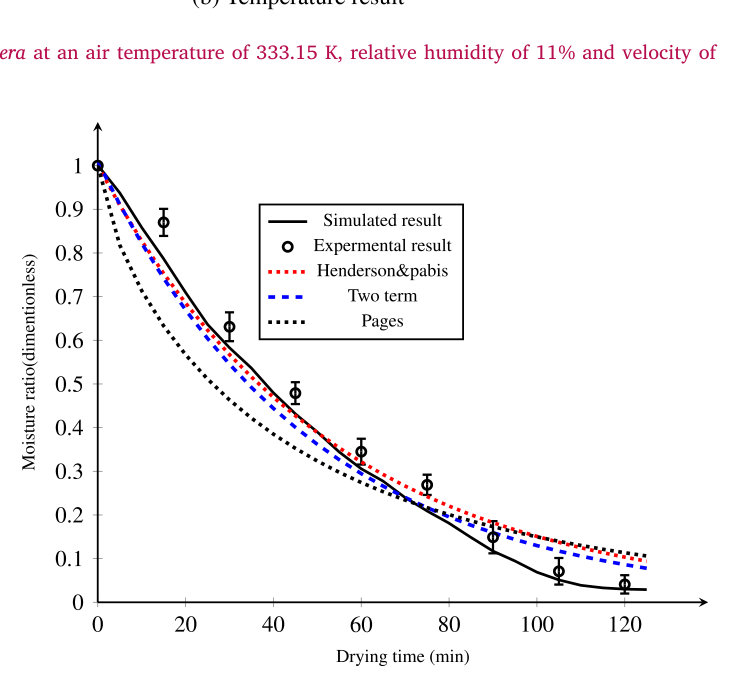
\includegraphics[width=0.5\textwidth]{figs2/fig14.png}
\caption{空气温度 333.15 K、风速 0.5 m\,s$^{-1}$ 下模拟干燥动力学与已知数学模型的比较。}
\label{fig:14}
\end{figure}

\section{结论}

本文建立了一个干燥过程中传热传质的耦合数学模型，用以研究英吉拉的干燥过程，预测了样品内部水分比与温度分布随时间的变化。基于仿真结果，较高的决定系数（水分与温度均 $R^2>0.95$）与较低的均方根误差（温度 RMSE $<3.5$ K，无量纲水分比 RMSE $<0.05$）表明实验与仿真之间吻合良好。可以得出结论：温度、风速及其交互作用对除水速率有显著影响（$p<0.05$）。该模型有助于更好地理解样品内部的传热与水分输运现象，本研究可安全地用于进一步的工程应用，并为食品干燥过程分析提供理论基础。

\vspace{8pt}
\noindent\textbf{作者贡献声明：}\textit{Alamrew B. Solomon}：构思并设计实验；开展实验；分析与解释数据；提供试剂、材料、分析工具或数据；撰写论文。\textit{Solomon W. Fanta}：构思并设计实验；分析与解释数据；提供试剂、材料、分析工具或数据；撰写论文。\textit{Mulugeta A. Delele}；\textit{Maarten Vanierschot}：分析与解释数据；撰写论文。

\noindent\textbf{资助声明：}本研究未获得公共、商业或非营利部门资助机构的专项资助。

\noindent\textbf{数据可用性声明：}数据可应要求提供。

\noindent\textbf{利益冲突声明：}作者声明无利益冲突。

\noindent\textbf{补充信息：}本文无补充信息。

\noindent\textbf{致谢：}作者感谢 Wollo 大学与 Bahirdar 大学提供的资金与技术支持，使本研究得以开展。

\section*{参考文献}
\addcontentsline{toc}{section}{参考文献}
\small
\begin{enumerate}
\item Aregawi, W., Defraeye, T., Saneinejad, S., Vontobel, P., Lehmann, E., Carmeliet, J., Verboven, P., Derome, D., Nicolai, B., 2014a. Understanding forced convective drying of apple tissue: combining neutron radiography and numerical modelling. Innov. Food Sci. Emerg. Technol. 24, 97--105.
\item Aregawi, W.A., Abera, M.K., Fanta, S.W., Verboven, P., Nicolai, B., 2014b. Prediction of water loss and viscoelastic deformation of apple tissue using a multiscale model. J. Phys. Condens. Matter 26 (46), 464111.
\item Arslan, D., Özcan, M.M., 2010. Study the effect of sun, oven and microwave drying on quality of onion slices. Lebensm.-Wiss. Technol. 43 (7), 1121--1127.
\item Ashagrie, Z., Abate, D., 2012. Improvement of injera shelf life through the use of chemical preservatives. Afr. J. Food Agric. Nutr. Dev. 12 (5), 6409--6423.
\item Ateeque, M., Mishra, R.K., Chandramohan, V., Talukdar, P., et al., 2014. Numerical modeling of convective drying of food with spatially dependent transfer coefficient in a turbulent flow field. Int. J. Therm. Sci. 78, 145--157.
\item Baur, F.J., Ensminger, L.G., 1977. The association of official analytical chemists (aoac). J. Am. Oil Chem. Soc. 54 (4), 171--172.
\item Bennamoun, L., Khama, R., Léonard, A., 2015. Convective drying of a single cherry tomato: modeling and experimental study. Food Bioprod. Process. 94, 114--123.
\item Berk, Z., 2018. Food Process Engineering and Technology. Academic Press.
\item Bird, R., Stewart, W., Lighfoot, E., 2001. Transport Phenomena, 2nd edn. 912 pp.
\item Bird, R.B., 2004. Five decades of transport phenomena. AIChE J. 50 (2), 273--287.
\item Bird, R.B., Stewart, W.E., Lightfoot, E.N., Klingenberg, D.J., 2015. Introductory Transport Phenomena. Wiley Global Education.
\item Bradstreet, R.B., 1954. Kjeldahl method for organic nitrogen. Anal. Chem. 26 (1), 185--187.
\item Cárcel, J., Garcia-Perez, J.V., Riera, E., Mulet, A., 2011. Improvement of convective drying of carrot by applying power ultrasound—influence of mass load density. Dry. Technol. 29 (2), 174--182.
\item Cengel, Y., Ghajar, A., 2011. Chapter eight: internal forced convection. In: Heat and Mass Transfer, Fundamentals and Applications. McGraw-Hill, New York, p. 489.
\item Cengel, Y.A., Boles, M.A., 2002. Thermodynamics: an engineering approach. Sea 1000, 8862.
\item Datta, A., 2007a. Porous media approaches to studying simultaneous heat and mass transfer in food processes. i: Problem formulations. J. Food Eng. 80 (1), 80--95.
\item Datta, A., 2007b. Porous media approaches to studying simultaneous heat and mass transfer in food processes. ii: Property data and representative results. J. Food Eng. 80 (1), 96--110.
\item Datta, A.K., Sahin, S., Sumnu, G., Keskin, S.O., 2007. Porous media characterization of breads baked using novel heating modes. J. Food Eng. 79 (1), 106--116.
\item Demir, V., Gunhan, T., Yagcioglu, A., Degirmencioglu, A., 2004. Mathematical modelling [and the experimental determination of the drying characteristics of some food products].
\item Doymaz, I., 2004. Drying kinetics of white mulberry. J. Food Eng. 61 (3), 341--346.
\item ElGamal, R., Ronsse, F., Pieters, J.G., 2017. [Modelling of heat and mass transfer during drying of food products].
\item Ertekin, C., Yaldiz, O., 2004. Drying of eggplant and selection of a suitable thin layer drying model. J. Food Eng. 63 (3), 349--359.
\item Feyissa, A.H., Gernaey, K.V., Adler-Nissen, J., 2013. [Uncertainty and sensitivity analysis of a multiphysics model for convection drying of a food product]. J. Food Eng.
\item Garau, M.C., Simal, S., Rosselló, C., Femenia, A., 2006. Effect of air-drying temperature on physico-chemical properties of dietary fibre and antioxidant capacity of orange (Citrus aurantium v. Canoneta) by-products. Food Chem.
\item Gebremariam, M.M., Zarnkow, M., Becker, T., 2014. Teff (Eragrostis tef) as a raw material for malting, brewing and manufacturing of gluten-free foods and beverages: a review. J. Food Sci. Technol. 51 (11), 2881--2895.
\item Gebremariam, M.M., Zarnkow, M., Becker, T., 2015. [Teff-based food products: a review].
\item Gulati, T., Datta, A.K., 2013. [Enabling computer-aided food process engineering: property estimation equations for transport phenomena-based models]. J. Food Eng.
\item Haard, N.F., 1999. [Fermented cereals: a global perspective]. FAO Agricultural Services Bulletin.
\item Horwitz, W., et al., 1970. Official Methods of Analysis of the Association of Official Analytical Chemists. AOAC, Washington, DC.
\item Horwitz, W., et al., 2010. Official Methods of Analysis of AOAC International, 18th edn. AOAC International, Gaithersburg, MD.
\item Hussain, M.A., Dincer, I., 2003. [Numerical simulation of two-dimensional heat and moisture transfer during drying of a rectangular object]. Dry. Technol.
\item Karim, M.A., Hawlader, M.N.A., 2005. [Mathematical modelling and experimental investigation of tropical fruits drying]. Int. J. Heat Mass Transf.
\item Kasiramar, G., 2019. [Determination of fat content by Soxhlet method].
\item Khan, M.I.H., et al., 2020. [CFD simulation of drying chamber for food drying].
\item Kumar, C., Karim, M.A., Joardder, M.U.H., 2014. [Intermittent drying of food products: a critical review]. J. Food Eng.
\item Kumar, C., et al., 2012. [Heat and mass transfer modelling of drying of food products].
\item Kuznetsov, A.V., Nield, D.A., 2013. [The Cheng-Minkowycz problem for natural convective boundary layer flow in a porous medium saturated by a nanofluid]. Int. J. Heat Mass Transf.
\item Law, C.L., et al., 2016. [Drying of food products: modelling and simulation].
\item Lemus-Mondaca, R., et al., 2013. [Modelling and simulation of drying of food products].
\item Marcotte, M., et al., 2008. [Thermophysical properties of food products].
\item Neela, S., Fanta, S.W., 2020. [Review on nutritional composition of teff (Eragrostis tef)].
\item Omolola, A.O., Jideani, A.I.O., Kapila, P.F., 2014. [Modeling microwave drying kinetics of banana (Musa acuminata)].
\item Pasban, A., et al., 2017. [CFD modelling of drying of food products].
\item Pham, N.D., et al., 2020. [CFD analysis of airflow and heat transfer in a drying chamber].
\item Satheesh, N., Fanta, S.W., 2018. [Review on the nutritional and functional properties of teff].
\item Shahari, N.B., 2012. [Heat and mass transfer modelling of food drying].
\item Shemishere, T., et al., 2018. [Thermal properties of teff-based food products].
\item Shen, L., et al., 2020. [Heat and mass transfer modelling of drying of porous food materials].
\item Telis-Romero, J., et al., 1998. [Thermophysical properties of food products].
\item Tesfay, Y., et al., 2014. [Injera: the traditional Ethiopian flatbread].
\item Tripathy, P.P., Kumar, S., 2008. [Modelling of drying of food products].
\item Tunckal, C., Doymaz, I., 2020. [Drying kinetics of food products: modelling and simulation].
\item Tzempelikos, D.A., et al., 2015. [Heat and mass transfer modelling of drying of food products].
\item Vásquez-Parra, J.C., et al., 2013. [Effect of drying on the physicochemical and nutritional properties of food products].
\item Villa-Corrales, L., et al., 2010. [Heat and mass transfer during drying of food products].
\item Yu, et al., 2020. [Convective heat and mass transfer coefficients in drying].
\item Zhang, J., Datta, A.K., 2004. [Some considerations in modeling of moisture transport in heating of hygroscopic porous materials]. Dry. Technol.
\item Zielinska, M., Markowski, M., 2010. [Air drying characteristics and moisture diffusivity of carrots]. Chem. Eng. Process.
\end{enumerate}

\end{document}
